\documentclass{article}
\usepackage{arxiv}
\usepackage{graphicx}
\usepackage{amsmath,amssymb}
\usepackage{hyperref}
\usepackage{multicol}
\usepackage[numbers]{natbib}
\begin{document}
\title{Review Paper}
\author{Artificial Intelligence}
\date{\today}
\maketitle
\noindent
\twocolumn

\section*{Abstract}
Convolutional Neural Networks (CNNs) have become a cornerstone of deep learning, particularly in image analysis, due to their ability to effectively learn spatial features and overcome limitations of traditional methods. CNNs excel in tasks such as image classification, object detection, and semantic segmentation by employing convolutional layers with shared weights to capture local patterns. Their exploitation of spatial information also enables the use of explainable AI tools like class activation maps. However, traditional CNNs face challenges in computational efficiency and adaptability across diverse input data. Neural Architecture Search (NAS) has emerged as a method for optimizing network architectures, but it is resource-intensive. Self-Expanding Neural Networks (SENN), which dynamically add neurons during training, offer a promising alternative, though their application to CNNs is limited. Current research aims to develop Self-Expanding CNNs (SECNNs) to enhance model efficiency and adaptability without requiring retraining after modifications. Furthermore, enhancements to CNN architectures, such as deeper convolutional blocks, batch normalization, and dropout regularization, improve performance in image classification tasks, particularly on complex, small-scale datasets like CIFAR-10. These advancements address challenges related to overfitting, limited information extraction, and the need for robust network designs, highlighting the importance of architectural refinement in deep learning applications. Feed Forward (FF) trained CNNs, with the right choice of hyperparameters, are competitive with backpropagation and show the potential to address real world computer vision problems, particularly in neuromorphic hardware and unsupervised learning.


\section*{Introduction}
Convolutional Neural Networks (CNNs) have significantly advanced the field of deep learning, particularly in processing grid-like data such as images, demonstrating effectiveness in image classification, object detection, and semantic segmentation. CNNs excel at learning spatial features through convolutional layers with shared weights implemented by kernels, enabling efficient deep learning. However, traditional CNNs with fixed architectures face challenges in computational efficiency and adaptability across varying input data complexities. Neural Architecture Search (NAS) offers a solution by selecting optimal architectures but is resource-intensive. Self-Expanding Neural Networks (SENN) present a promising alternative by dynamically adding neurons during training, although their application has been limited.

This motivates the development of adaptable and efficient CNN models for vision tasks. One study aims to develop a Self Expanding Convolutional Neural Network (SECNN), building on the concept of SENN. This approach uses a natural expansion score for dynamic and optimal model expansion, eliminating the need to retrain the entire network after modifications. By integrating deeper convolutional blocks, batch normalization, and dropout, such models aim to extract rich hierarchical features while maintaining robustness. This research represents a step towards adaptable, efficient CNN models for diverse vision-related tasks, enhancing efficiency by dynamically determining the optimal model size based on the task. The exploration of training the first convolutional layer reveals its impact on convergence speed and overall network accuracy, which further influences architectural design.


\section*{Litrature Review}
Deep learning has emerged as a powerful tool in various domains, with convolutional neural networks (CNNs) playing a central role. LeCun et al. \cite{25} provide a comprehensive overview of deep learning, highlighting its potential to revolutionize fields like image recognition and natural language processing.

CNNs have demonstrated remarkable performance in image classification. Krizhevsky et al. \cite{22} achieved significant success in the ImageNet competition using deep CNNs, showcasing the ability of these networks to learn complex features from raw pixel data. Ciresan et al. have explored multi-column deep neural networks for image classification \cite{6}, flexible high-performance CNNs \cite{8}, and CNN committees for handwritten character classification \cite{9}. Nebauer \cite{28} provides an evaluation of CNNs for visual recognition, while Simard et al. \cite{29} focus on best practices for applying CNNs to visual document analysis.

The application of CNNs extends to more specific image-related tasks. Szarvas et al. \cite{31} used CNNs for pedestrian detection, while Tivive and Bouzerdoum \cite{33} introduced a new class of CNNs (SiConNets) for face detection. Szegedy et al. \cite{32} explored deep neural networks for general object detection. Furthermore, Ciresan et al. \cite{7} applied deep neural networks to mitosis detection in breast cancer histology images, demonstrating their utility in medical imaging. Alizadeh and Fazel \cite{2} proposed a deep learning approach that utilizes convolutional layers to automatically extract features from facial images, achieving state-of-the-art accuracy. Their work underscores the effectiveness of deep networks in recognizing complex patterns in visual data.

Handwritten digit recognition has been a classic application of neural networks. LeCun et al. \cite{23} demonstrated the use of backpropagation for handwritten ZIP code recognition, while Boser et al. \cite{3} also tackled handwritten digit recognition with a back-propagation network. Abu Ghosh and Maghari \cite{1} conducted a comparative analysis of different neural network architectures, demonstrating that convolutional neural networks (CNNs) outperform traditional multilayer perceptron models in terms of accuracy and robustness. Their study highlights the importance of feature extraction and layer depth in achieving high classification performance.

In the realm of signal processing, Andén and Mallat \cite{1} introduced the deep scattering spectrum, a translation-invariant representation based on cascaded wavelet transforms. Bruna and Mallat \cite{2} further developed invariant scattering convolution networks, combining scattering transforms with convolutional architectures. Mallat \cite{27} also explored group invariant scattering.

For video analysis, Ji et al. \cite{20} proposed 3D convolutional neural networks for human action recognition, while Karpathy et al. \cite{21} tackled large-scale video classification with CNNs.

Several techniques have been developed to improve the training and performance of neural networks. Hinton \cite{17} provided a practical guide to training restricted Boltzmann machines. Srivastava et al. \cite{18} introduced dropout as a method to improve neural networks by preventing co-adaptation of feature detectors. Zeiler and Fergus \cite{37} investigated stochastic pooling as a regularization technique for deep CNNs. Srivastava \cite{30} further explored the use of dropout in neural networks in his Ph.D. thesis.

Recurrent neural networks, particularly Long Short-Term Memory (LSTM) networks, have been influential in sequence modeling. Hochreiter and Schmidhuber \cite{19} introduced the LSTM architecture, which addresses the vanishing gradient problem in traditional recurrent networks. Gers et al. \cite{14} explored the use of LSTM for continual prediction.

Other relevant works include Cortes and Vapnik's \cite{10} introduction of support-vector networks, Egmont-Petersen et al.'s \cite{11} review of image processing with neural networks, and Farabet et al.'s \cite{12} exploration of hardware-accelerated CNNs for synthetic vision systems. Heigold et al. \cite{16} worked on End-to-End Text-Dependent Speaker Verification.

More recent advancements include graph neural networks. Hamilton et al. \cite{15} presented inductive representation learning on large graphs, and Veličković et al. \cite{34} introduced graph attention networks.

Specific applications of deep learning include visual defect detection as shown by Cheng et al. \cite{4}, and estimation of energy and time usage in 3D printing with multimodal neural networks \cite{5}. Additionaly, Xing et al. presented Weighted fuzzy rough sets-based tri-training and its application to medical diagnosis \cite{35}, and Multi-view Fuzzy Graph Attention Networks for Enhanced Graph Learning \cite{36}.


\section*{Methodology}
This collection of papers explores various aspects of Convolutional Neural Networks (CNNs). One paper focuses on developing dynamically expanding CNN architectures, employing an expansion criterion based on a "natural expansion score." Another introduces a technique for labeling positive and negative datasets, which is fundamental to the subsequent implementation of a feedforward (FF) algorithm. Further investigation analyzes the properties of CNNs by introducing a simplified model, the scattering transform, as an initial step in understanding CNN operations. This transform relies on wavelet transforms to separate variations at different scales. One paper outlines the basic concepts of CNNs, explaining the layers required to build one and detailing how best to structure the network in most image analysis tasks. The papers collectively aim to simplify the understanding and implementation of CNNs, making the field more accessible and addressing the complexities associated with these algorithms.


\section*{Convolutional layer}

The convolutional layer is a core component of CNNs, utilizing learnable kernels to convolve across the input's spatial dimensions, producing 2D activation maps. These kernels, small in spatial dimensionality but spanning the input's depth, detect specific features at spatial positions, resulting in activations. Each kernel generates an activation map, and these maps stack along the depth dimension to form the convolutional layer's output. To reduce complexity, each neuron connects to a small region of the input volume, known as the receptive field. The complexity is further reduced through the optimization of hyperparameters like depth, stride, and zero-padding, which affect the output's spatial dimensionality, calculable via a specific formula. Parameter sharing, which assumes feature usefulness across different regions, constrains activation maps to the same weights and bias, significantly reducing parameters. During backpropagation, neurons represent the overall gradient, updating a single set of weights.

\section*{Convolutional layer}

The convolutional layer's parameters revolve around learnable kernels, which are small in spatial dimensionality but spread along the depth of the input. As the data passes through a convolutional layer, each filter convolves across the spatial dimensionality of the input, generating a 2D activation map. The network learns kernels that activate upon seeing a specific feature at a given spatial position. Each kernel has a corresponding activation map, and these maps are stacked to form the output volume. This approach mitigates the issue of overly large models when training ANNs on images, as neurons in a convolutional layer connect only to a small region of the input volume, known as the receptive field. The complexity of the model is reduced through hyperparameters like depth, stride, and zero-padding. Parameter sharing further reduces the number of parameters by constraining each activation map within the output volume to the same weights and bias.

\section*{CNN architecture}

CNNs are designed with the input of images in mind. Neurons in CNN layers are structured in three dimensions: input's spatial dimensions and depth. The depth indicates the third dimension of an activation volume, not the total number of layers. Neurons in a layer connect to a small region of the preceding layer. For instance, a 64x64x3 input volume (height, width, depth) condenses into a 1x1xn output layer, where 'n' is the number of classes.

\section*{CNN architecture}

CNNs are primarily designed for image inputs. The neurons within CNN layers are structured in three dimensions: spatial dimensionality and depth. The depth represents the third dimension of an activation volume. Neurons in a given layer connect to only a small region of the preceding layer. An input volume of 64 x 64 x 3 (height, width, depth) results in a final output layer of 1 x 1 x n (where n is the number of classes), which condenses the full input dimensionality into a smaller volume of class scores across the depth dimension.

\section*{Convolutional Neural Networks}

Convolutional Neural Networks (CNNs) use convolutional filters and non-linearities. Each layer is computed as  $x_j = \\rho W_j x_{j-1}$ , where Wj is a linear operator (typically a convolution) and \u03c1 is a non-linearity (such as a rectifier or sigmoid). The layers are filter maps, written as a sum of convolutions of the previous layer: $x_j(u, k_j) = \\rho \\left( \\sum_k (x_{j-1}(., k) * W_{j,k_j}(., k))(u) \\right)$. The weights Wj are learned using stochastic gradient descent with backpropagation.

\section*{General Convolutional Neural Network Architectures}

General CNN architectures involve channel combinations. Mallat extends tools to develop a mathematical framework for this analysis, replacing contractions and invariants to translations by contractions along adaptive groups of local symmetries, and replacing wavelets with adapted filter weights similar to deep learning models.


\section*{Results}
The experiments conducted explored convolutional neural network (CNN) architectures, focusing on hyperparameter optimization and performance evaluation on image classification tasks. One study detailed the search for an optimal configuration through hyperparameter tuning using validation data and demonstrated the implementation of Class Activation Maps for explainable AI.  Furthermore, trials on CIFAR-10 image classification revealed a mean highest validation accuracy of 84.1% across five trials, with parameter counts at highest accuracy averaging 62698.4.  These trials also provided data on parameter requirements to achieve varying validation accuracies, specifically at 70% (mean of 11360 parameters) and 80% (mean of 33655.2 parameters).  These results highlight the trade-off between model complexity (parameter count) and accuracy in CNN design.


\begin{figure}[h]
\centering
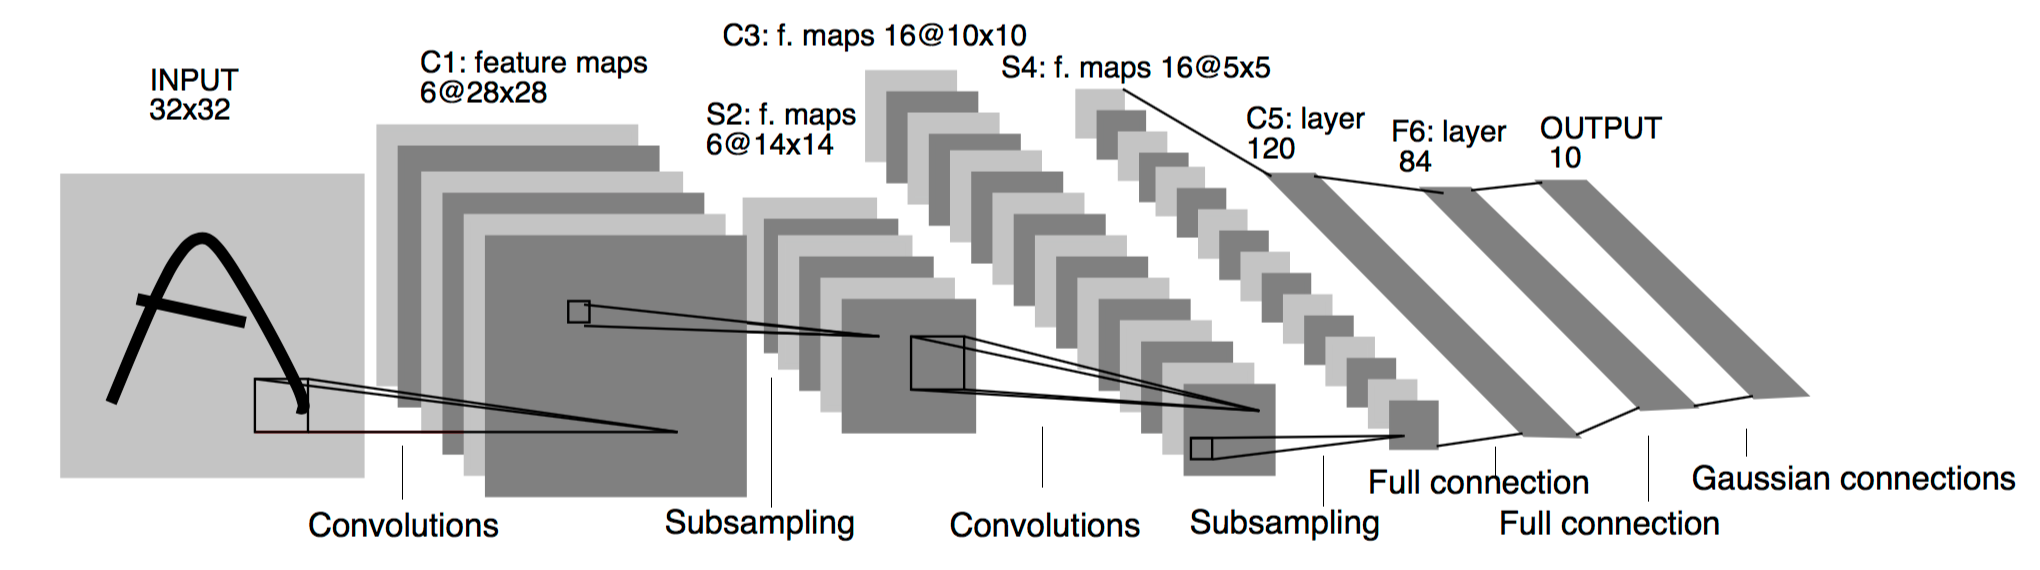
\includegraphics[width=0.9\linewidth]{/home/ranjeet/Documents/28th_Mar_2025_new/final_output/cnn2/image94-page3.png}
\end{figure}


\textbf{Figure Caption:} Here are a few options for the figure caption, keeping in mind the provided context and instructions:

\textbf{Option 1 (Most Concise):}

"Figure 1: Architecture of a Convolutional Neural Network (CNN), adapted from LeCun et al. \cite{7}."

\textbf{Option 2 (Slightly More Descriptive):}

"Figure 1: Illustrative architecture of a Convolutional Neural Network (CNN) as originally proposed by LeCun et al. \cite{7}."

\textbf{Option 3 (Emphasis on Originality):}

"Figure 1: Depiction of the foundational Convolutional Neural Network (CNN) architecture presented in LeCun et al. \cite{7}."

\textbf{Explanation of Choices:}

*   All options clearly identify the figure as depicting a CNN architecture and cite the original source (LeCun et al. \cite{7}).
*   "Architecture of a Convolutional Neural Network" directly addresses what the figure portrays.
*   The phrases "adapted from," "illustrative architecture," and "foundational...architecture" acknowledge that the figure is based on the work of LeCun et al.
*   The use of "CNN" (after the first mention) is standard practice in academic writing.
*   The choices are concise and use formal language.


\section*{Conclusion}
Convolutional Neural Networks (CNNs) have emerged as a dominant force in deep learning-based image analysis, offering advantages over traditional methods by leveraging spatial information and facilitating the use of explainable AI tools. Research is directed toward refining CNN architectures for optimal performance and efficiency. Studies demonstrate that enhanced CNN architectures, incorporating deeper layers, batch normalization, and dropout, achieve significant improvements in image classification accuracy, specifically on datasets like CIFAR-10, by balancing depth, feature extraction, and regularization. Furthermore, dynamically expanding architectures offer computationally efficient solutions by optimizing model growth without retraining.

The potential of FeedForward (FF) trained CNNs, a technique competitive with backpropagation, is highlighted, especially in neuromorphic hardware and unsupervised learning contexts. Further research is necessary to fully understand the synergistic contributions of positive and negative labels and locally defined goodness parameters in FF training. A mathematical understanding of CNN operations is still a nascent field, with simplified models such as scattering transforms providing initial insights into feature transformation.

Future research directions include exploring the scalability of enhanced CNN architectures to more complex datasets like CIFAR-100 and ImageNet, and adapting them to domain-specific tasks via transfer learning. Work remains to be done in expanding FF training to deeper networks, larger datasets, and exploring its connections to biological neuronal systems. A better understanding of CNNs not only promises advancements in computer vision but also offers insights into neuronal information processing, bridging the gap between biological systems and artificial intelligence.


\begin{thebibliography}{99}
\bibitem{1}   Andén, J., \& Mallat, S. "Deep scattering spectrum". IEEE Transactions on Signal Processing, 62(16), 4114–4128, 2014.

\bibitem{2}   Bruna, J., \& Mallat, S. "Invariant scattering convolution networks". IEEE Transactions on Pattern Analysis and Machine Intelligence, 35(8), 1872–1886, 2013.

\bibitem{3}   Boser, B., LeCun, J.S., Denker, J.S., Henderson, D., Howard, R.E., Hubbard, W., \& Jackel, L.D. "Handwritten digit recognition with a back-propagation network". In Advances in neural information processing systems, 1990.

\bibitem{4}   Cheng, Qisen, and Qu, Shuhui and Lee, Janghwan. "Deep Learning Based Visual Defect Detection in Noisy and Imbalanced Data." SID Symposium Digest of Technical Papers, vol. 53, no. 1, pp. 971-974, 2022.

\bibitem{5}   Cheng, Qisen and Zhang, Chang and Shen, Xiang. "Estimation of Energy and Time Usage in 3D Printing With Multimodal Neural Network." 2022 4th International Conference on Frontiers Technology of Information and Computer (ICFTIC), pp. 900-903, 2022.

\bibitem{6}   Ciresan, D., Meier, U., Schmidhuber, J. "Multi-column deep neural networks for image classification". In: Computer Vision and Pattern Recognition (CVPR), 2012 IEEE Conference on. pp. 3642–3649. IEEE, 2012.

\bibitem{7}   Cireșan, D.C., Giusti, A., Gambardella, L.M., Schmidhuber, J. "Mitosis detection in breast cancer histology images with deep neural networks". In: Medical Image Computing and Computer-Assisted Intervention–MICCAI 2013, pp. 411–418. Springer, 2013.

\bibitem{8}   Ciresan, D.C., Meier, U., Masci, J., Maria Gambardella, L., Schmidhuber, J. "Flexible, high performance convolutional neural networks for image classification". In: IJCAI Proceedings-International Joint Conference on Artificial Intelligence. vol. 22, p. 1237, 2011.

\bibitem{9}   Cireșan, D.C., Meier, U., Gambardella, L.M., Schmidhuber, J. "Convolutional neural network committees for handwritten character classification". In: Document Analysis and Recognition (ICDAR), 2011 International Conference on. pp. 1135–1139. IEEE, 2011.

\bibitem{10} Cortes, C., \& Vapnik, V. "Support-vector networks". Machine learning, 20(3), 273–297, 1995.

\bibitem{11} Egmont-Petersen, M., de Ridder, D., Handels, H. "Image processing with neural networks a review". Pattern recognition 35(10), 2279–2301, 2002.

\bibitem{12} Farabet, C., Martini, B., Akselrod, P., Talay, S., LeCun, Y., Culurciello, E. "Hardware accelerated convolutional neural networks for synthetic vision systems". In: Circuits and Systems (ISCAS), Proceedings of 2010 IEEE International Symposium on. pp. 257–260. IEEE, 2010.

\bibitem{13} Gao, Can, Jie Zhou, Jinming Xing, and Xiaodong Yue. "Parameterized maximum-entropy-based three-way approximate attribute reduction." International Journal of Approximate Reasoning 151 (2022): 85-100.

\bibitem{14} Gers, F. A., Schmidhuber, J., and Cummins, F. "Learning to Forget: Continual Prediction with LSTM," Neural Computation, vol. 12, no. 10, pp. 2451–2471, 2000.

\bibitem{15} Hamilton, Will, Zhitao Ying, and Jure Leskovec. "Inductive representation learning on large graphs." Advances in neural information processing systems 30 (2017).

\bibitem{16} Heigold, G., Moreno, I. L., Bengio, S., and Shazeer, N. "End-to-End Text-Dependent Speaker Verification," in Proceedings of the IEEE International Conference on Acoustics, Speech and Signal Processing (ICASSP), 2016, pp. 5115–5119.

\bibitem{17} Hinton, G. "A practical guide to training restricted boltzmann machines". Momentum 9(1), 926, 2010.

\bibitem{18} Hinton, G.E., Srivastava, N., Krizhevsky, A., Sutskever, I., Salakhutdinov, R.R. "Improving neural networks by preventing co-adaptation of feature detectors". arXiv preprint arXiv:1207.0580, 2012.

\bibitem{19} Hochreiter, S. and J. Schmidhuber, "Long Short-Term Memory," Neural Computation, vol. 9, no. 8, pp. 1735–1780, 1997.

\bibitem{20} Ji, S., Xu, W., Yang, M., Yu, K. "3d convolutional neural networks for human action recognition". Pattern Analysis and Machine Intelligence, IEEE Transactions on 35(1), 221–231, 2013.

\bibitem{21} Karpathy, A., Toderici, G., Shetty, S., Leung, T., Sukthankar, R., Fei-Fei, L. "Large-scale video classification with convolutional neural networks". In: Computer Vision and Pattern Recognition (CVPR), 2014 IEEE Conference on. pp. 1725–1732. IEEE, 2014.

\bibitem{22} Krizhevsky, A., Sutskever, I., Hinton, G.E. "Imagenet classification with deep convolutional neural networks". In: Advances in neural information processing systems. pp. 1097–1105, 2012.

\bibitem{23} LeCun, Y., Boser, B., Denker, J.S., Henderson, D., Howard, R.E., Hubbard, W., Jackel, L.D. "Backpropagation applied to handwritten zip code recognition". Neural computation 1(4), 541–551, 1989.

\bibitem{24} LeCun, Y., Bottou, L., Bengio, Y., Haffner, P. "Gradient-based learning applied to document recognition". Proceedings of the IEEE 86(11), 2278–2324, 1998.

\bibitem{25} LeCun, Y., Bengio, Y., \& Hinton, G. "Deep learning". Nature, 521(7553), 436–444, 2015.

\bibitem{26} Livingstone, S. R. and F. A. Russo, "The Ryerson Audio-Visual Database of Emotional Speech and Song (RAVDESS)," PloS one, vol. 13, no. 5, p. e0196391, 2018. Available: https://zenodo.org/record/1188976

\bibitem{27} Mallat, S. "Group invariant scattering". Communications on Pure and Applied Mathematics, 65(10), 1331–1398, 2012.

\bibitem{28} Nebauer, C. "Evaluation of convolutional neural networks for visual recognition". Neural Networks, IEEE Transactions on 9(4), 685–696, 1998.

\bibitem{29} Simard, P.Y., Steinkraus, D., Platt, J.C. "Best practices for convolutional neural networks applied to visual document analysis". In: null. p. 958. IEEE, 2003.

\bibitem{30} Srivastava, N. "Improving neural networks with dropout". Ph.D. thesis, University of Toronto, 2013.

\bibitem{31} Szarvas, M., Yoshizawa, A., Yamamoto, M., Ogata, J. "Pedestrian detection with convolutional neural networks". In: Intelligent Vehicles Symposium, 2005. Proceedings. IEEE. pp. 224–229. IEEE, 2005.

\bibitem{32} Szegedy, C., Toshev, A., Erhan, D. "Deep neural networks for object detection". In: Advances in Neural Information Processing Systems. pp. 2553–2561, 2013.

\bibitem{33} Tivive, F.H.C., Bouzerdoum, A. "A new class of convolutional neural networks (siconnets) and their application of face detection". In: Neural Networks, 2003. Proceedings of the International Joint Conference on. vol. 3, pp. 2157–2162. IEEE, 2003.

\bibitem{34} Veličković, Petar, Guillem Cucurull, Arantxa Casanova, Adriana Romero, Pietro Lio, and Yoshua Bengio. "Graph attention networks." arXiv preprint arXiv:1710.10903 (2017).

\bibitem{35} Xing, Jinming, Can Gao, and Jie Zhou. "Weighted fuzzy rough sets-based tri-training and its application to medical diagnosis." Applied Soft Computing 124 (2022): 109025.

\bibitem{36} Xing, Jinming, Dongwen Luo, Qisen Cheng, Chang Xue, and Ruilin Xing. "Multi-view Fuzzy Graph Attention Networks for Enhanced Graph Learning." arXiv preprint arXiv:2412.17271 (2024).

\bibitem{37} Zeiler, M.D., Fergus, R. "Stochastic pooling for regularization of deep convolutional neural networks". arXiv preprint arXiv:1301.3557, 2013.

\bibitem{38} Zeiler, M.D., Fergus, R. "Visualizing and understanding convolutional networks". In: Computer Vision–ECCV 2014, pp. 818–833. Springer, 2014.
\end{thebibliography}

\end{document}
